\section{Analysis}\hfill

In order to determine if the model is able to provide useful insight into a practical physics analysis, we attempt to reconstruct the Higgs mass from DiHiggs decaying to 4b events with a non-resonant 4b background. The non-resonant 4b sample has a 60GeV pTB filter applied at generation level to ensure the kinematics of each sample are indistinguishable. Therefore, the only difference between these samples is the the resonant mass peak that appears in the DiHiggs sample and the flat background from the non-resonant 4b sample.

Using the results of the Efrac and Mfrac model, we are able to apply jet corrections and see 

\begin{figure}[h!]
    \centering
    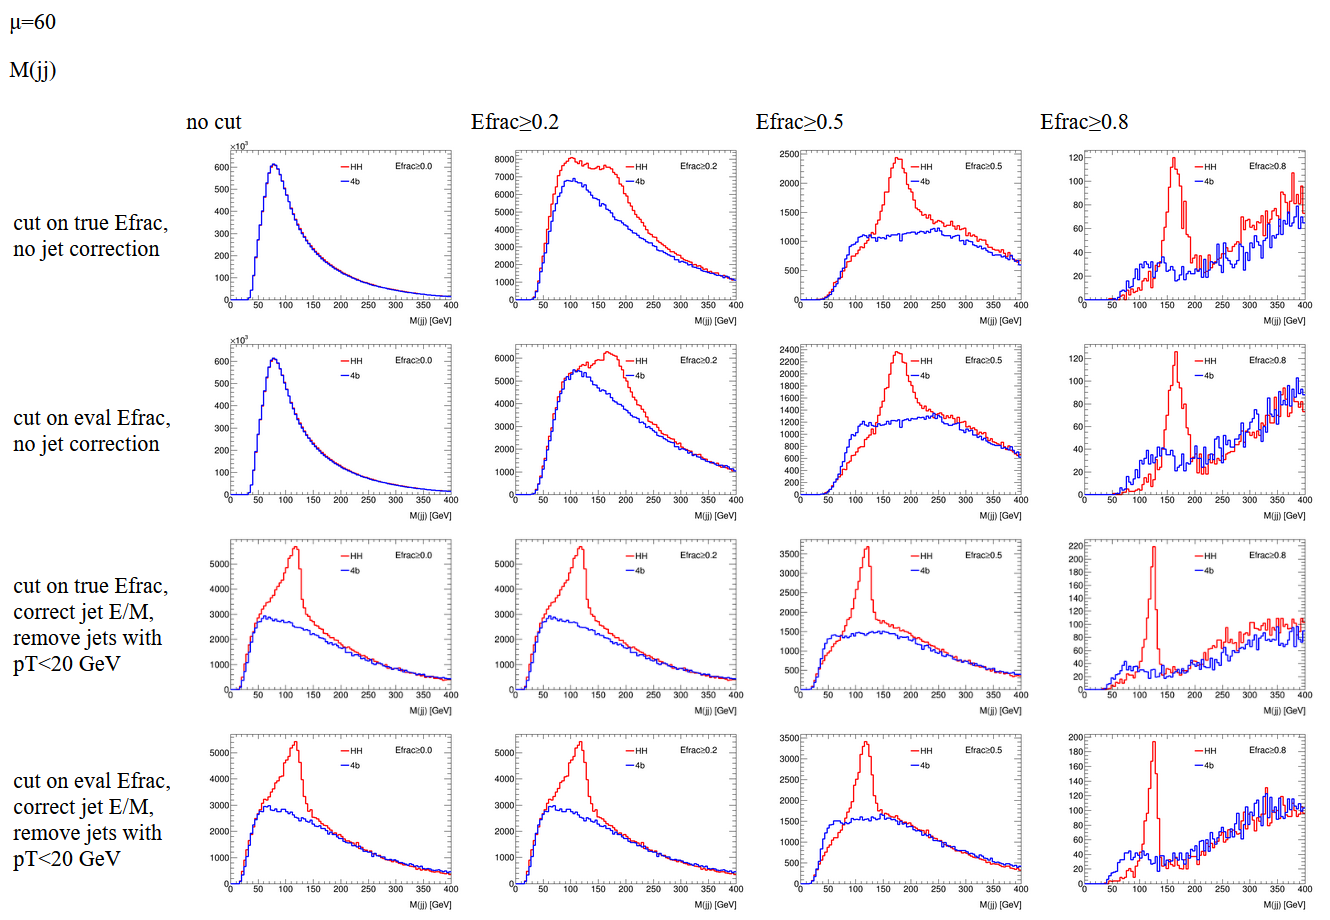
\includegraphics[width=1\linewidth]{tmp.png}
    \caption{Physics Analysis Results}
\end{figure}
